% -*- coding: utf-8 -*-
\documentclass{beamer}
%\documentclass[handout]{beamer} %打印版本
\usepackage{ctex} %注意这个宏包
\usepackage{algorithmic}
\usepackage{algorithm}
\usepackage{subfig}
%\renewcommand{\algorithmicrequire}{\textbf{输入:}}
%\renewcommand{\algorithmicensure}{\textbf{输出:}}
%\floatname{algorithm}{算法}
%\usepackage{beamerthemesplit}
%
%
% 打开PDF后直接全屏
\hypersetup{pdfpagemode={FullScreen}}
%\beamertemplateballitem

\mode<presentation>
{
\usetheme{Antibes}
%\usetheme{default}
%\usetheme{Frankfurt}
%\usetheme{Berkeley}
%\usetheme{Goettingen}

\usecolortheme{seahorse}
}

%\usepackage{pgfpages}
%%\pgfpagesuselayout{2 on 1}[a4paper,border shrink=3mm]
%\pgfpagesuselayout{4 on 1}[a4paper,landscape,border shrink=3mm]

%%usetheme{Madrid}
%%这里还可以选择别的主题:Bergen, Boadilla, Madrid, AnnArbor, CambridgeUS, Pittsburgh, Rochester, Warsaw, ...
%%有导航栏的Antibes, JuanLesPins, Montpellier, ...
%%有内容的Berkeley, PaloAlto, Goettingen, Marburg, Hannover, ...
%%有最小导航栏的Berlin, Ilmenau, Dresden, Darmstadt, Frankfurt, Singapore, Szeged, ...
%%有章和节表单的Copenhagen, Luebeck, Malmoe, Warsaw, ...
%
%%usecolortheme{default}
%%设置内部颜色主题(这些主题一般改变block里的颜色);这个主题一般选择动物来命名
%%这里还可以选择别的颜色主题,如默认的和有特别目的的颜色主题default,structure,sidebartab,全颜色主题albatross,beetle,crane,dove,fly,seagull,wolverine,beaver
%
%%usecolortheme{orchid}
%%设置外部颜色主题(这些主题一般改变title里的颜色);这个主题一般选择植物来命名
%%这里还可以选择别的颜色主题,如默认的和有特别目的的颜色主题lily,orchid,rose
%
%%usecolortheme{whale}
%%设置字体主题;这个主题一般选择海洋动物来命名
%%这里还可以选择别的颜色主题,如默认的和有特别目的的颜色主题whale,seahorse,dolphin
%
%%usefonttheme{professionalfonts}
%%类似的还可以定义structurebold,structuresmallcapsserif,professionalfonts
%
%
%% 控制 beamer 的风格,可以根据自己的爱好修改
%%usepackage{beamerthemesplit} %使用 split 风格
%%usepackage{beamerthemeshadow} %使用 shadow 风格
%%usepackage[width=2cm,dark,tab]{beamerthemesidebar}
%

\title{符号属性数据的半监督聚类与属性选择}
\author{王文涛}
\date{\today}
\begin{document}

\frame{\titlepage}

\section*{目录}

\frame{\tableofcontents}

\section{聚类与属性选择概述}

\subsection*{聚类}

\frame {\frametitle{聚类}
聚类问题就是在没有任何数据的先验信息下对数据进行聚类分析,它是一种有效的分析数据结构的手段。
\begin{itemize}
\item<1-> 基于划分,基于层次,基于密度,基于网格
\item<2-> 符号属性数据聚类
\begin{itemize}
  \item 基于类型转换
  \item 基于概率统计
  \item 基于相异测度
\end{itemize}

\end{itemize} }

\subsection*{属性选择}

\frame {\frametitle{属性选择}
属性选择是指在初始属性集中选择出一个属性子集,可以像属性全集一样用来正确区分数据集中的每个数据对象。
\begin{itemize}
\item<1-> 过滤模型、封装模型和混合模型
\item<2-> 属性评价方法:距离度量、信息度量、依赖性度量
\item<3-> 搜索策略:启发式、穷尽式、随机式
\end{itemize}}

\subsection*{符号属性半监督学习}

\frame {\frametitle{符号属性半监督学习}
针对无监督聚类和属性选择已经成为机器学习领域中的重要的研究方向,但是,半监督聚类和属性选择研究得相对较少,特别是符号属性数据,因此符号属性数据的半监督聚类和属性选择具有研究价值。
}



\section{权值投票的半监督聚类集成}


\subsection*{权值投票的半监督聚类集成}
\frame {\frametitle{权值投票的半监督聚类集成}
\begin{figure}
  \centering
  % Requires \usepackage{graphicx}
  \center
  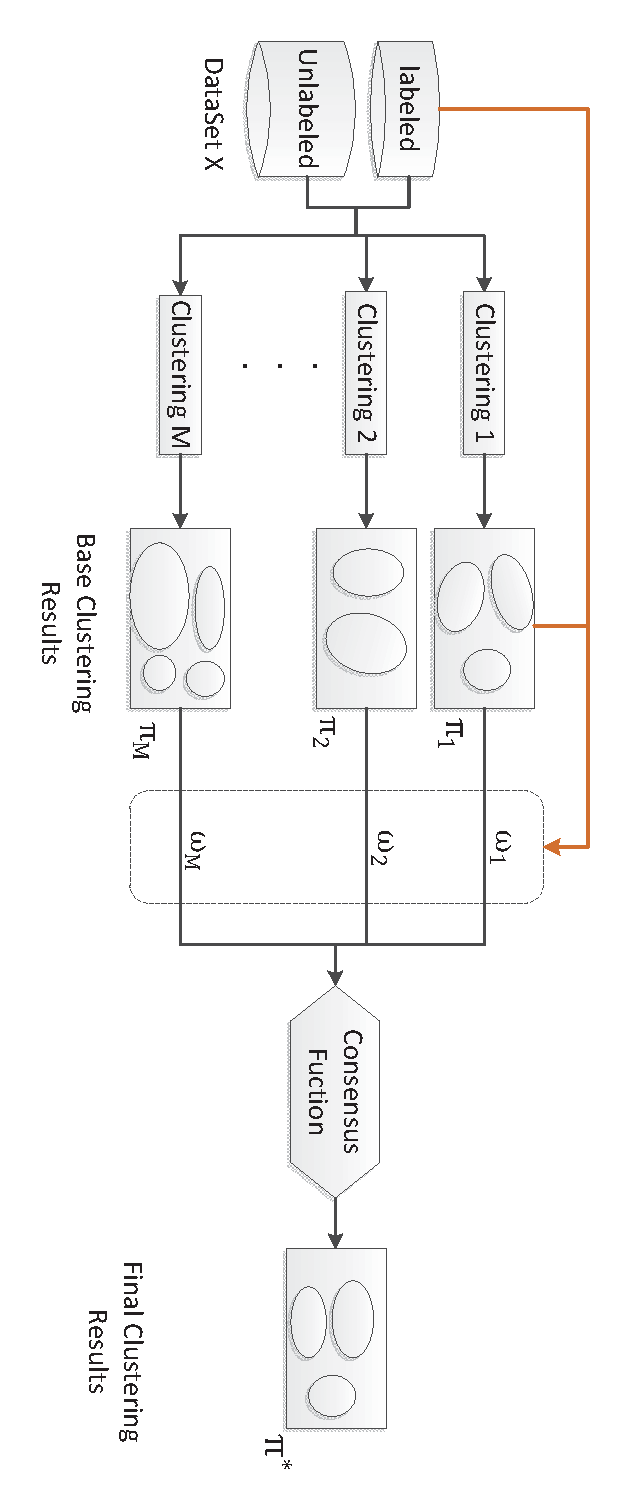
\includegraphics[width=0.38\textwidth,angle=90]{fig1.eps}\\
\end{figure}
}

\subsection*{权值投票的半监督聚类集成算法}
\frame {\frametitle{权值投票的半监督聚类集成算法}
\begin{itemize}
\item<1-> 生成不同的聚类结果:k-Modes算法初始点不同
\item<2-> 权值产生:有监督部分和无监督部分(NMI)
\item<4-> 一致性函数:标签对齐,权值投票
\begin{itemize}
  \item W\_Voting
  \item S\_W\_Voting
  \item Random\_W\_Voting
  \item Random\_S\_W\_Voting
\end{itemize}

\end{itemize}

}

\subsection*{对比实验}
\frame {

\begin{figure}
\subfloat[ACC-Alpha]{
\begin{minipage}[b]{0.33\textwidth}
\centering
\includegraphics[width=1\textwidth]{./part1/Promoters-alpha-AC.eps}
\end{minipage} }
\subfloat[ACC-Ensize]{
\begin{minipage}[b]{0.33\textwidth}
\centering
\includegraphics[width=1\textwidth]{./part1/Promoters-ensize-AC.eps}
\end{minipage} }
\subfloat[ACC-Lpercent]{
\begin{minipage}[b]{0.33\textwidth}
\centering
\includegraphics[width=1\textwidth]{./part1/Promoters-per-AC.eps}
\end{minipage} }

\subfloat[NMI-Alpha]{
\begin{minipage}[b]{0.33\textwidth}
\centering
\includegraphics[width=1\textwidth]{./part1/Promoters-alpha-NMI.eps}
\end{minipage} }
\subfloat[NMI-Ensize]{
\begin{minipage}[b]{0.33\textwidth}
\centering
\includegraphics[width=1\textwidth]{./part1/Promoters-ensize-NMI.eps}
\end{minipage} }
\subfloat[NMI-Lpercent]{
\begin{minipage}[b]{0.33\textwidth}
\centering
\includegraphics[width=1\textwidth]{./part1/Promoters-per-NMI.eps}
\end{minipage} }
\end{figure}


}

\section{基于分裂重组合的半监督聚类}

\subsection*{分裂重组合的半监督聚类}
\frame {\frametitle{基于分裂重组合的半监督聚类}
\begin{figure}
  \centering
  % Requires \usepackage{graphicx}
  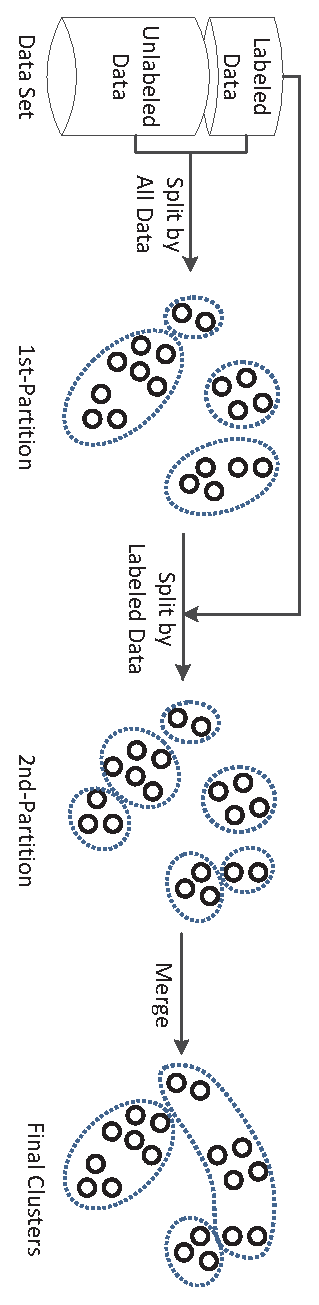
\includegraphics[width=0.25\textwidth,angle=90]{fig2.eps}\\
 % \caption{基于分裂组合的半监督聚类示意图}\label{fig:chapter4:fig1}
\end{figure}

}

\subsection*{分裂与组合}

\frame {\frametitle{分裂组合策略}
\begin{itemize}
\item<1-> 分裂策略:属性等价关系与类标等价关系形成划分
\item<2-> 组合策略:

\begin{figure}
\subfloat[Single]{
\begin{minipage}[b]{0.2\textwidth}
\centering\label{fig:chapter5:hc:dis:single}
\includegraphics[width=1\textwidth]{single-link.eps}
\end{minipage} }
\subfloat[Complete]{
\begin{minipage}[b]{0.2\textwidth} \label{fig:chapter5:hc:dis:complete}
\centering
\includegraphics[width=1\textwidth]{complete-link.eps}
\end{minipage} }
\subfloat[Average]{
\begin{minipage}[b]{0.2\textwidth} \label{fig:chapter5:hc:dis:average}
\centering
\includegraphics[width=1\textwidth]{average-link.eps}
\end{minipage} }
\subfloat[Mean]{
\begin{minipage}[b]{0.2\textwidth} \label{fig:chapter5:hc:dis:mean}
\centering
\includegraphics[width=1\textwidth]{mean-link.eps}
\end{minipage} }
\end{figure}

\end{itemize}

}


\subsection*{距离函数}
\frame {\frametitle{对象间距离函数}

假设数据集$X=X^L\bigcup X^U\in R^m$,其中$X^L$为有类标数据,$X^U$为无类标数据,$m$为符号属性的个数,则$x_i,x_j\in X$的半监督差异测度定义为
\begin{equation}\label{equ:chapter4:hc:semidis}
  d(x_i,x_j)\left\{
  \begin{array}{ll}
    -m & x_i\in X^L \wedge x_j\in X^L \wedge d_i=d_j \\
    m & x_i\in X^L \wedge x_j\in X^L \wedge d_i\neq d_j\\
    \sum^m_{l=1}\delta(x_{il},x_{jl})  & otherwise
  \end{array}
  \right.
\end{equation}

}


\subsection*{对比实验}
\frame {

\begin{figure}
\subfloat[ACC-Lpercent]{
\begin{minipage}[b]{0.5\textwidth}
\centering
\includegraphics[width=1\textwidth]{./part2/Hayes-per-AC.eps}
\end{minipage} }
\subfloat[NMI-Lpercent]{
\begin{minipage}[b]{0.5\textwidth}
\centering
\includegraphics[width=1\textwidth]{./part2/Hayes-per-NMI.eps}
\end{minipage} }
\end{figure}

}




\section{最小冗余最大相关半监督属性选择}

\subsection*{相关性与冗余性}
\frame {\frametitle{最小冗余最大相关半监督属性选择}
\begin{itemize}
\item<1-> 属性评价:


假设数据集$X= X^L\bigcup X^U$,$A=\{a_1,a_2,\ldots,a_m\}$为$m$ 个属性的集合,对于有类标数据$X^L$,$d$为决策属性,属性$a_i$ 的相关性与冗余性定义为
\begin{equation}
\begin{split}
  D(a_i)= & MI^L(a_i,d) \\
   R(a_i,S_m)= & MI^{U}(a_i,S_m)+\sum_{a_j\in S_m}\frac{MI(a_i,a_j)}{|S_m|}
\end{split}
\end{equation}

\item<2-> 搜索策略:贪心式算法优化的约束条件为:
\begin{equation}
  \max_{a_j\in \{A-S_{m-1}\}}\bigg[D(a_j)-R(a_j,S_{m-1})\bigg]
\end{equation}
\end{itemize}
}


\subsection*{对比实验}
\frame {

\begin{itemize}
\item<1-> 半监督属性选择分类效果
\begin{figure}
\subfloat[CART-Alpha]{
\begin{minipage}[b]{0.45\textwidth}
\centering
\includegraphics[width=1\textwidth]{./part3/Credit_part3_eva_cart_alpha.eps}
\end{minipage} }
\subfloat[CART-Lpercent]{
\begin{minipage}[b]{0.45\textwidth}
\centering
\includegraphics[width=1\textwidth]{./part3/Credit_part3_eva_cart_per.eps}
\end{minipage} }
\end{figure}
\end{itemize}

}

%\frame {\frametitle{最小冗余最大相关半监督属性选择}
%
%\begin{algorithm}[H]
%\begin{algorithmic}[1]
%\REQUIRE 决策系统$DS=<U,A\cup D,V,f>$
%\ENSURE 条件属性$A$相对于决策决策属性$D$的一个相对约简$B\in RED_D(A)$
%\STATE $B=\varnothing$
%\STATE $a_i=\argmax_{a_i\in A-B}SIG(a_i,B,D)$
%\STATE $B=B\cup \{a_i\}$
%\WHILE{$POS_B(D)\neq POS_A(D)$}
%\STATE $a_i=\argmax_{a_i\in A-B}SIG(a_i,B,D)$
%\STATE $B=B\cup \{a_i\}$
%\ENDWHILE
%\RETURN $B\in RED_D(A)$
%\end{algorithmic}
%\end{algorithm}
%}

\section{基于耦合依赖度的半监督属性选择}

\subsection*{粗糙集}
\frame {\frametitle{正域及依赖度}
假设给定一个知识表达系统$S=<U,A,V,f>$,$\forall X\subseteq U$和$B\subseteq A$,子集$X$关于$B$的下近似和上近似分别是
\begin{equation}\label{equ:chapter6:roughset:lowapp}
\begin{split}
  \underline{B}(X)= & \{x|\forall x\in U,[x]_B\subseteq X\} \\
   \overline{B}(X)= & \{x|\forall x\in U,[x]_B\cap X\neq \varnothing\}
\end{split}
\end{equation}
$POS_B(X)=\underline{B}(X)$称为$X$关于$B$的正域。
\begin{equation}\label{equ:chapter6:roughset:dep}
  \gamma_B(D)=\frac{POS_B(D)}{|U|}=\frac{\bigg|\bigcup_{X\in U/D}\underline{B}(X)\bigg|}{|U|}
\end{equation}
为$D$依赖于$B$的程度,记作$B\Rightarrow_k D$
}

\subsection*{耦合依赖度}
\frame {\frametitle{耦合依赖度的半监督属性选择算法}
\begin{itemize}
\item<1-> 属性评价:

假设给定一个知识表达系统$S=<U,A,V,f>$,$a_i,a_j\subseteq A$,耦合依赖度,相关性及冗余性定义为:
\begin{equation}
  daulDep(a_i,a_j)=\frac{POS_{a_i}(a_j)+POS_{a_j}(a_i)}{2|U|}
\end{equation}
\begin{equation}\label{equ:chapter6:rel}
  Rel(a_i,d)=daulDep^L(a_i,d)
\end{equation}
\begin{equation}\label{equ:chapter6:red}
  Red(a_i,a_j)=daulDep(a_i,a_j)
\end{equation}
\item<2-> 搜索策略:
如果属性的相关性大于其对于已选属性中每个属性的冗余性,我们就将它加入的属性选择子集中,反之,就将它丢弃。
\end{itemize}
}

\subsection*{对比实验}
\frame {

\begin{itemize}
\item<1-> 半监督属性选择分类效果
\begin{figure}
\subfloat[CART-Lpercent]{
\begin{minipage}[b]{0.45\textwidth}
\centering
\includegraphics[width=1\textwidth]{./part4/Heart-cleveland_part4_eva_cart_per.eps}
\end{minipage} }
\subfloat[CART-Lpercent]{
\begin{minipage}[b]{0.45\textwidth}
\centering
\includegraphics[width=1\textwidth]{./part4/WDBC_part4_eva_cart_per.eps}
\end{minipage} }
\end{figure}
\item<2-> 半监督聚类与属性选择结合验证:\\
实验结果表明经过SemiMRMR算法和DualPOS算法属性选择后的数据大都能保持属性全集上的半监督聚类效果。
\end{itemize}
}
\subsection*{}%加星号不在目录里

\frame{
  \frametitle{\subsecname}
 % \begin{columns}
 % \column{3cm}
  %\column{4cm}
  %  Thank you for your time!
 % \column{3cm}
 % \end{columns}

  \begin{center}
   \includegraphics[width=100mm]{Thankyou.pdf}\\
   \textcolor[rgb]{0.00,0.00,1.00}{浙江大学计算机学院}\\
   \textcolor[rgb]{0.00,1.00,0.00}{E-mail:wwtzju@qq.com}\\
\end{center}


}


\end{document}
